\documentclass[12pt]{report}
\usepackage[spanish, activeacute]{babel}
\usepackage[top=2.75cm,bottom=2.50cm,left=3.00cm,right=2.50cm]{geometry}
\usepackage[utf8]{inputenc}  
\usepackage{enumerate}
\usepackage{graphicx}



\begin{document}
	\setlength{\topmargin}{-0.5in}
	\pagestyle{empty}
	\begin{center}
		\textbf{
			\vspace{-0.7em}
			ESCUELA SUPERIOR POLITÉCNICA DEL LITORAL
		}
		\line(1,0){380}\\		
		\scriptsize{FACULTAD DE INGENIERÍA EN ELECTRICIDAD Y COMPUTACIÓN}
	\end{center}

	\begin{center}
		\vspace{2.5em}
		\Huge{\textbf{\\PROYECTO FINAL}}
	\end{center}	

	\begin{center}
		\Huge{\textbf{\\Recopilación de Trabajos II Término 2012	\vspace{1em}}}
	\end{center}
	\begin{center}
		\Huge{\textbf{\\Ana Arias	\vspace{1em}}}
		\\ acarias@espol.edu.ec
	\end{center}
	\begin{center}
		\Huge{\textbf{\\Lenguajes de Programación\vspace{1em}}}
	\end{center}	
	\begin{center}
		\Huge{\textbf{\\Ing. Javier Tibau	\vspace{1em}}}
		\\ jtibau@espol.edu.ec
		\\ jtibau@fiec.espol.edu.ec
	\end{center}	



\chapter*{Agradecimientos}
\addcontentsline{toc}{chapter}{Agradecimientos} 
\markboth{AGRADECIMIENTOS}{AGRADECIMIENTOS} % encabezado 
 
Quiero agradecer a mis compañeros de grupo y compañeros del aula, ya que entre todos compartimos conocimientos y buenas experiencias.
También quiero agradecer a mi profesor de Lenguajes de Programación Ing. Javier Tibau por darnos todos los retos de este semestre.

\chapter*{Resumen} 
\addcontentsline{toc}{chapter}{Resumen} 
\markboth{RESUMEN}{RESUMEN} % encabezado

Este documento contiene las descripciones y experiencias de los proyectos realizados en la materia Lenguajes de Programación dirigida por el Ing. Javier Tibau.

\tableofcontents


%---------------------------------------------------------------------------------------------------------------------------------
%--------------------------------------------------------------GITHUB!------------------------------------------------------
%---------------------------------------------------------------------------------------------------------------------------------
\chapter{Herramienta GitHub\label{capitulouno}}

	\begin{center}
		\begingroup
			
\includegraphics[width=0.27\textwidth]{imagenes_usuario/git.png}
		\endgroup
	\end{center}


	\begingroup
		\large{
			\textbf{
			           \newline
			           \newline
				Experiencias y Anécdotas: GitHub
				\newline
				\newline
			}
		}
	\endgroup
Mi experiencia con GitHub ha sido buena, esta herramienta en verdad mejoró la comunicación en los trabajos con mi grupo; lo que más me agradó es que podemos estar actualizados con respecto a las modificaciones en los archivos que nos tocó hacer de forma grupal, y por lo tanto se evita el compartir documentos frecuentemente a través de otra herramienta y la creación de un sinfín de documentos que contienen en realidad lo mismo.
\newline
\newline	
Considero Github como una red social, ya que podemos estar conectados con nuestros compañeros y compartir información, y además de ser social, es seria ya que a partir de esta herramienta se pueden encontrar trabajos muy interesantes de distintas personas, dicho material puede ser muy útil.
\newline
\newline	
Con respecto a su uso, lo considero sencillo y mecánico; al principio es un poco difícil aprender cómo se utiliza pero después se vuelve costumbre ya que los procedimientos para subir archivos, para crear repositorios, para modificarlos es en realidad muy mecánico.
\newline
Esta herramienta es una buena opción para dar a conocer nuestros trabajos en internet, y seguramente la seguiré utilizando en el futuro.
\newline
\newline
Mi experiencia con Github a lo largo del semestre pasó de ser mala, a regular y finalmente a muy buena. Esto tiene mucho que ver por toda la practica que tuvimos que tener con esta herramienta, ya que la utilizamos en todos los proyectos.
El uso de la herramienta Github se facilitó mucho cuando empecé a utilizar su interfaz.
\newline
	\begin{center}
		\begingroup
			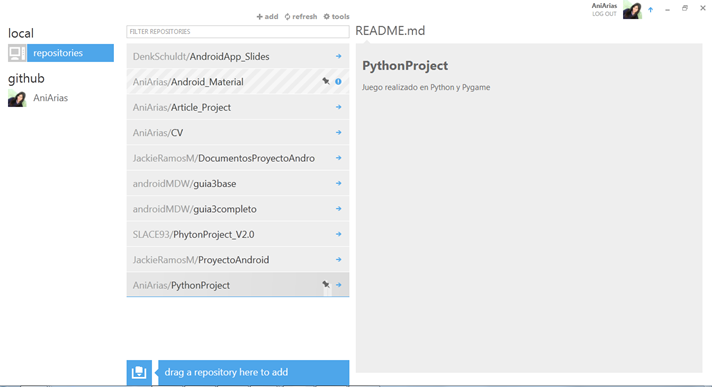
\includegraphics[width=0.8\textwidth]{imagenes_usuario/git2.png}
\newline
\newline
		\endgroup
	\end{center}

	\begin{center}
		\begingroup
			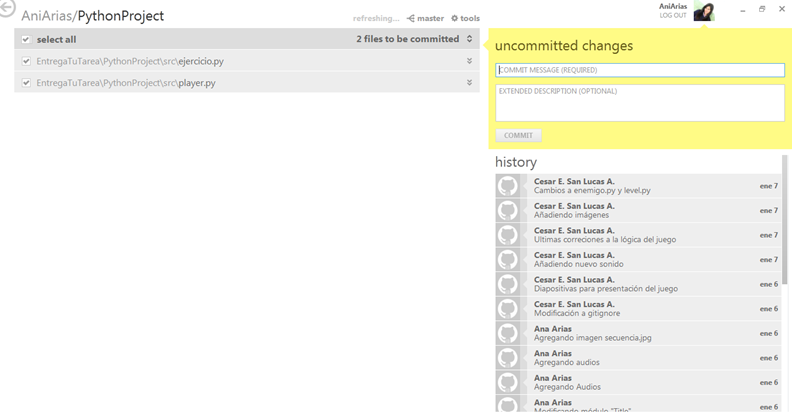
\includegraphics[width=0.8\textwidth]{imagenes_usuario/git3.png}
\newline
\newline
		\endgroup
	\end{center}

La interfaz de Github permite realizar commits de manera mucho mas rápida y mas detallada; me pareció mu interesante la rapidez con que se actualizaban los proyectos cada vez que se modificaba algo.
Recomendaría utilizar la interfaz de GitHub para las personas que recién empiecen a utilizar esta herramienta.
\newline
\newline
Seguiré utilizandola para futuros proyectos y en mi vida profesional.

 \ref{capitulouno}















\end{document}